
%(BEGIN_QUESTION)
% Copyright 2006, Tony R. Kuphaldt, released under the Creative Commons Attribution License (v 1.0)
% This means you may do almost anything with this work of mine, so long as you give me proper credit

A water pump bypass valve has a full-open C$_{v}$ rating of 120.  If the pump outputs a flow of 1500 GPM of water at a differential pressure (outlet pressure - inlet pressure) of 68 PSID, what will be the total water flow output by the system when the bypass valve is 100\% open?

$$\includegraphics[width=15.5cm]{i01817x01.eps}$$


\underbar{file i01817}
%(END_QUESTION)





%(BEGIN_ANSWER)

$Q_{outlet}$ = 510.5 GPM
 
%(END_ANSWER)





%(BEGIN_NOTES)

It should be noted that this method of flow control on a water pump is much preferable to locating the valve in-line with the pump discharge.  Water pumps may be damaged if their discharge is blocked, and this is what will happen when an in-line valve ever closes.  Bypass valves do not cause this same problem.

%INDEX% Final Control Elements, valve: sizing

%(END_NOTES)


